\documentclass[11 pt]{article}  
\usepackage[utf8]{inputenc}
\usepackage{amsmath}
\usepackage{amsfonts}
\usepackage{amssymb}
\usepackage{graphicx}
\usepackage{mathrsfs}
\usepackage{upref,amsthm,amsxtra,exscale}
\usepackage{stmaryrd}
\usepackage{cite}
\usepackage[colorlinks=true,urlcolor=blue,
citecolor=red,linkcolor=blue,linktocpage,pdfpagelabels,bookmarksnumbered,bookmarksopen]{hyperref}


\newcommand\blue[1]{{\color{blue}\textbf{#1}}}

\newcommand\inter[1]{\llbracket #1\rrbracket}



\usepackage[cm]{fullpage}

\usepackage{subcaption}
\usepackage{caption}
\usepackage{cleveref}


\newtheorem{theorem}{Theorem}[section]
\newtheorem{corollary}[theorem]{Corollary}
\newtheorem{remark}[theorem]{Remark}
\newtheorem{lemma}[theorem]{Lemma}
\newtheorem{proposition}[theorem]{Proposition}
\newtheorem{definition}[theorem]{Definition}
\newtheorem{example}[theorem]{Example}
\numberwithin{equation}{section}

\usepackage{enumitem}

\def\N{\mathbb{N}}

\def\r{\mathbb{R}}
\def\diam{\operatorname{diam}}
\def\dist{\operatorname{dist}}
\def\rn{\mathbb{R}^N}
\def\rt{\mathbb{R}^3}
\def\z{\mathbb{Z}}
\def\zn{\mathbb{Z}^N}
\def\n{\mathbb{N}}
\def\cc{\mathbb{C}}
\def\eps{\varepsilon}
\def\rh{\rightharpoonup}
\def\io{\int_{\Omega}}
\def\irn{\int_{\r^N}}
\def\irt{\int_{\rt}}
\def\vp{\varphi}
\def\tilde{\widetilde}
\def\cD{\mathcal{D}}
\def\cI{\mathcal{I}}
\def\cJ{\mathcal{J}}
\def\cM{\mathcal{M}}
\def\cN{\mathcal{N}}
\def\cO{\mathcal{O}}
\def\cU{\mathcal{U}}
\def\cV{\mathcal{V}}
\def\cW{\mathcal{W}}

\newcommand{\norm}[2]{{\left\|#1\right\|}_{#2}}
\newcommand{\fl}[2]{(-d_x^2)^{#1}#2}
\newcommand{\rfl}[2]{A^{#1}_{\Omega}#2}
\newcommand{\hp}[1]{\hphantom{#1}}
\newcommand{\cns}{c_{N,s}}
\newcommand{\ccs}{c_{1,s}}
\newcommand{\ffl}[2]{(-d_x^{\,2})^{#1}#2}
\newcommand{\flh}[2]{\frac{1}{\Gamma(-s)}\int_0^{+\infty}\Big(e^{t\Delta}#2 - #2\Big)\frac{dt}{t^{1+#1}}}
\newcommand{\kernel}[1]{|x-y|^{#1}}
\newcommand{\dkj}{\delta_{kj}}
\newcommand{\intr}[1]{\underset{#1}{\int}}
\newcommand{\Do}[1]{D_{#1}}
\newcommand{\Hs}{H^s_0(\Omega)}
\newcommand{\ue}[1]{#1^{\,\varepsilon}}
\newcommand{\xHdot}[1]{\dot{H}^{#1}}
\newcommand{\ha}[2]{\mathbf{H}_{#1}^{#2}}
\newcommand{\lhi}{\mathcal{L}_i^h}
\newcommand{\NN}{\mathbb{N}}
\newcommand{\ZZ}{\mathbb{Z}}
\newcommand{\RR}{\mathbb{R}}
\newcommand{\CC}{\mathbb{C}}
\newcommand{\TT}{\mathbf{T}}
\newcommand\mesh{\mathfrak{M}}


\newcommand{\weH}[1]{\mathbb H^{#1}(\Omega;\ell)}


%Alberto's defs
\def\R{\mathbb{R}}
\def\S{\mathbb{S}}
\def\cP{\mathcal{P}}
\def\cM{\mathcal{M}}
\def\cL{\mathcal{L}}
\def\mH{\mathbb{H}}
\def\cE{\mathcal{E}}
\def\cC{\mathcal{C}}
\def\cH{\mathcal{H}}
\def\weakto{\rightharpoonup}
\def\d{\textnormal{d}}


\def\sideremark#1{\ifvmode\leavevmode\fi\vadjust{\vbox to0pt{\vss% the remark
 \hbox to 0pt{\hskip\hsize\hskip1em%                          will appear only
 \vbox{\hsize2.1cm\tiny\raggedright\pretolerance10000%          on the side
  \noindent #1\hfill}\hss}\vbox to15pt{\vfil}\vss}}}%
\newcommand{\edz}[1]{\sideremark{#1}}
    
    \usepackage{color}
\usepackage[dvipsnames]{xcolor}
\newcommand{\B}[1]{{\color{red} #1}}  %for paper content
\newcommand{\Bc}[1]{{\color{red}\textbf{#1}}}  %for comments
\newcommand{\SJ}[1]{{\color{ForestGreen} #1}}  %for paper content
\newcommand{\SJc}[1]{{\color{green}\textbf{#1}}}  %for comments

\usepackage{tikz}
\usepackage{pgfplots}
\usepackage{pgfplotstable}
\usetikzlibrary{positioning}
\usepackage{booktabs}
%\usepackage{subfig}


\newcommand{\weakly}{\rightharpoonup}

\title{FEM for 1D-problems involving the logarithmic Laplacian: error estimates and numerical implementation}

\author{V\'ictor Hern\'andez-Santamar\'ia\footnote{The work of V. Hern\'andez-Santamar\'ia is supported by the program ``Estancias Posdoctorales por México para la Formación y Consolidación de las y los Investigadores por México'' of CONAHCYT (Mexico). He also received support from Projects A1-S-17475 and A1-S-10457 of CONAHCYT and by UNAM-DGAPA-PAPIIT grants IN109522, IN104922, and IA100324 (Mexico).} \and
 Sven Jarohs
 \and
Alberto Salda\~{n}a\footnote{ A. Saldaña is supported  by  
CONAHCYT grants A1-S-10457 and  CBF2023-2024-116 (Mexico) and by UNAM-DGAPA-PAPIIT grant IA100923 (Mexico).}\and
Leonard Sinsch
}

\date{}

\begin{document}

\begin{center}
 Answers to the referee reports.
\end{center}

We thank all the referees for the careful reading of our manuscript and for all the helpful comments and suggestions that substantially improved our paper. Below we include a point-by-point answer to each of the reports.  For clarity, we have copied all the items from the reports and answered them one by one below.


\subsubsection*{Report 1}


\section*{Main remarks}

\begin{enumerate}
    \item \emph{Given the low regularity of the problem and its solutions, it is not clear to me why the authors use linear finite elements instead of piecewise constants. Actually, the computation of the stiffness matrix seems to be simpler for \(P_{0}\) elements, and it seems convergence rates would not deteriorate by such a choice. Is there any reason to prefer \(P_{1}\) elements over \(P_{0}\) in this problem?}

    Our main reason to use $P_1$ elements in this work is to connect our work with previous works in the literature for the fractional Laplacian, where $P_1$ elements have been used. In this sense, we can use the stiffness matrix that was calculated before, take its derivative, and show that this procedure gives an stiffness matrix for the logarithmic Laplacian.

    Nevertheless, we agree with the referee that using $P_0$ elements is somewhat simpler and we also agree that probably teh convergence rates would not change much.  We do plan to do this in future work.



    \item \emph{The choice of the interpolation operator is not clear to me. The authors use a sort of localized \(L^{2}\) interpolation operator, and to have the constant-preservation property (3.10), they need to modify the standard Lagrange basis at the interval endpoints. It seems to me that what is required on the interpolation is its localization (this property is exploited in Lemma 3.5) and stability in \(L^{\infty}\) (this is used in Proposition 3.8, but it seems to me that it can be weakened to stability in \(L^{p}\) for some \(p>2\)). Therefore, I wonder why not using Clement interpolation on the whole mesh (including the domain boundary). Note also that for \(P_{0}\) elements the choice of the interpolation operator would be simpler, as one can just use localized averages and these in turn satisfy the two desired properties.}

    Indeed, we only require the constant-preservation property (3.10), the localization bonds (Lemma 3.5) and the stability (Proposition 3.8). This can be achieved with different choices of interpolators and basis. With the referee's comment, we now realize that a modification of the basis can be confusing and it is, in fact, not needed. One can use  the standard basis, plus an adjustment to the interpolator. In this revised version we have implemented this change: we now use the standard basis and modified the interpolator accordingly.

    Regarding the use of other interpolators and other finite elements, we agree that this is possible, but we do not believe that this would make an important improvement in our results or that would greatly simplify the computations. Our main motivation to use $P_1$ elements is to link this work with previous work on the fractional Laplacian where $P_1$ elements have been used.


    \item \emph{The authors prove logarithmic convergence rates (in energy norm), and claim that numerical evidence support that this is the case. While I agree with the statement if applied to the \(L^{\infty}\) norm, I disagree with it when applied to the \(L^{2}\) norm. The results in Figure 2 and Tables 2 and 3 seem to indicate convergence with order \(h^{1/2}\) in \(L^{2}(\Omega)\). This is consistent with the fact that the solution of the problem is continuous and therefore in \(\bigcap_{\epsilon>0}H^{1/2-\epsilon}(\mathbb{R})\). In the same vein, in my opinion Remark 6.1 is not correct, as I think the integral in the right-hand side does not have a sign. I suggest to rewrite the discussion about convergence in pages 17-18.}

%     We disagree on the claim that the solution always belongs to $\bigcap_{\epsilon>0}H^{1/2-\epsilon}(\mathbb{R})$.  For instance, let
%     \begin{align*}
%      \mathcal{H}_0^{s}((0,2)):=\{u\in H^{s}(\r)\::\: u=0\text{ in }\r\backslash (0,2)\}.
%     \end{align*}
% In
% \begin{center}
%  V. Hernández-Santamaría, L.F. López Ríos, and A. Saldaña, ''Optimal boundary regularity and a Hopf-type lemma for Dirichlet problems involving the logarithmic Laplacian'', Discrete and Continuous Dynamical Systems (2025),
% \end{center}
% it is shown that the function
% \begin{align*}
%  u(x):=\frac{1}{\sqrt{\ln(\frac{x}{2})}}\varphi(x)\chi_{[0,\infty)}
% \end{align*}
% (here $\varphi\in C^\infty_c(\r)$, $\varphi=1$ in $[0,1]$, and $\chi_{[0,\infty]}$ is the characteristic function in $[0,\infty)$) is a classical solution of
% \begin{align*}
%  L_\Delta u =f\quad \text{ in }[0,2],\qquad u=0\quad \text{ in }\r\backslash[0,2],
% \end{align*}
% for some $f\in L^\infty([0,2])$. Now, let $C$ denote possibly different constants independent of $\eps$; then,
% \begin{align*}
%  \|u\|_{\mathcal{H}_0^{1/2-\eps}((0,2))}^2
%  &=C\int_{\r}\int_{\r}\frac{|u(x)-u(y)|^2}{|x-y|^{1+2(\frac{1}{2}-\eps)}}\, dy\, dx
%  \geq C\int_{-1}^0\int_{0}^1\frac{1}{|\ln (\frac{y}{2})||x-y|^{2-2\eps}}\, dy\, dx\\
% & =C\int_{0}^1\frac{1}{|\ln (\frac{y}{2})|}\int_{0}^1\frac{1}{(x+y)^{2-2\eps}}\, dx\, dy
%  \geq C\int_{0}^{\frac{1}{2}}\frac{y^{2\eps-1}}{|\ln (y)|}\, dy\to \infty
% \end{align*}
% as $\eps\to 0$.
%
%

We find this remark very interesting. As far as we know, the claim that solutions belong to \(\bigcap_{\epsilon>0}H^{1/2-\epsilon}(\mathbb{R})\) has not been shown (although this is indeed true for the few explicit cases that are known). It would be very interesting to find estimates in this direction that can be used to show a better convergence rate. However, we do not believe that these estimates are immediate or easy to obtain.

We also agree that there is enough reasonable doubt regarding the convergence rate of the $L^2$ norm and that the numerical experiments that we provide do not settle this question. We have emphasized this in the new version. Moreover, we also agree that Remark 6.1 is not correct and it has been removed.

\end{enumerate}

\section*{Other comments and questions}

\begin{enumerate}
    \item[4.] \emph{I wonder why in the definition of weak solutions (page 3, line 6) the authors assume \(f\in L^{2}(\Omega)\) instead of \(f\in\mathbb{H}(\Omega)^{\prime}\).}

    We agree that one can take \(f\in\mathbb{H}(\Omega)^{\prime}\). In this paper we do not intend to obtain the most generality everywhere. Since this work is the first FEM analysis for the logarithmic Laplacian, we prefer to fix a simplified framework, to identify the key questions, to answer them in the best way possible with the estimates at our disposal, and to pose the main open questions that in our opinion can unlock the general theory for these problems.

    \item[5.] \emph{Clarify the sentence in page 5, lines 1-2: the entries of the matrix \({\mathcal{A}}_{h}^{L}\) only depend on \(h\), but the matrix itself does depend on \(L\), as its size obviously changes if one modifies \(L\).}

    Here we mean that the matrix \({\mathcal{A}}_{h}^{L}\) does not depend on $h$ \emph{and} on the interval $L$ in the following sense: for two different intervals splitted in the same number of subintervles one would obtain the same matrix \({\mathcal{A}}_{h}^{L}\).

    We have changed the wording in this part of the introduction.

    \item[6.] \emph{The first part of Lemma 3.2 does not use that \(v\in\mathbb{H}(\Omega)\); this hypothesis can be weakened to \(v\in L^{2}(\Omega)\).}

    We agree and we have changed this as suggested.

    \item[7.] \emph{I find definitions (3.13) and (3.14) a little confusing. I think it would be clearer if these sets were defined explicitly in terms of indices. The sets \(I_{i}\) seem to be related with the sets \(T_{i}\) in Lemma 3.12 (although the former are indices sets and the latter are subsets of \(\Omega\)) and that such sets are actually used already in Lemma 3.6, albeit without a definition. I think the paper would benefit if the authors unified the notation for these sets.}

    We have simplified the notation in this revised version, and now the definitions of $T_i$, $I_i$, and $I_i'$ are explicit.  Moreover, the relationship between $T_i$ and $I_i$ is now explicitly stated.

    \item[8.] \emph{The proof of Lemma 3.12 is almost the same than the proof of Lemma 3.6. The difference lies in the estimation of \(|b_{k}|\), namely, in whether using (3.22) or (3.32), and a very minor modification in the right-hand side of (3.30) with respect to (3.20). I suggest to shorten the proof of Lemma 3.12.}

 We agree with the referee. We have simplified the proof.

    \item[9.] \emph{I think the proofs of Lemmas 4.1 and Lemma 4.2 would become a little more clear if the authors made a few modifications.}
    \begin{itemize}
        \item \emph{Lemma 4.1 assumes a discrete inf-sup condition, which is clearly equivalent to the uniform well-posedness of the discrete problems, and Lemma 4.2 in turn gives a sufficient condition for such a hypothesis to hold. This is interesting, the sufficient condition boils down to the well-posedness of the continuous problem (which depends on the domain size) and having a sufficiently fine partition. I suggest to make this point explicit, adding a few lines between the two lemmas.}

        We agree and we have included this comment.

        \item \emph{I think it is convenient to use an \(h\) subindex to distinguish functions in \({\mathcal{V}}_{h}\) from arbitrary functions in \(\mathbb{H}(\Omega)\). The same comment applies to Proposition 7.2 as well.}

We agree with the referee and we have implemented the suggestion.

        \item \emph{In formula (4.3) I would change \(u_{h}\mapsto v_{h}\) to avoid confusion with the solution of the discrete problem.}

        We agree with the referee and we have implemented the suggestion.

        \item \emph{In the first sentence of the proof of Lemma 4.1, I think there is no need to take an arbitrary basis of \({\mathcal{V}}_{h}\), as one can simply take the finite element basis already introduced (and which is the one actually employed in practice).}

        We agree with the referee and we have implemented the suggestion.

        \item \emph{Isn't the assumption in Lemma 4.2 equivalent with alternative i) in Theorem 1.1?}

    Yes, it is equivalent. We have added a remark in this regard.

    \end{itemize}

    \item[10.] \emph{Proposition 4.3 does not quite belong to Section 4, as it does not involve the stability of the error. I think the authors decided to have it there because it is instrumental for the proof of Theorem 1.2, but I think it should be moved to the Introduction, after Theorem 1.1. Even though it can be a little strange to have a result proven in the introduction, the point of the paper is not the regularity of solutions and readership of CAMWA already know that regularity of solutions is one of the basic ingredients needed to prove convergence rates.}

    We agree with the referee.  We have relocated Proposition 4.3 in Section 2.2 (Variational Setting), right after the space $\mathbb H^{\beta}(\Omega)$ has been defined.


    \item[11.] \emph{Lemma 5.1 deals with the interesting fact that the stiffness matrices for the logarithmic Laplacian can be computed by differentiation with respect to \(s\) of the stiffness matrices for the fractional Laplacian. While in the paper the authors apply this result for a specific setting (intervals and uniform meshes) by direct differentiation, I think it would be interesting to consider its application in more general situations. In that sense, I wonder if the consistency error of replacing the derivative by a forward difference can be estimated. Namely, my question is what can be said about replacing \(L_{\Delta}\varphi_{i}\) by \(\frac{(-\Delta)^{s}\varphi_{i}-\varphi_{i}}{s}\) for small \(s\). I guess the error in \(L^{p}(\mathbb{R})\) should be linear in \(s\); is that correct?}

    It is true that
    \begin{align*}
     \left\|\frac{(-\Delta)^{s}\varphi_{i}-\varphi_{i}}{s}-L_{\Delta}\varphi_{i}\right\|_{L^p}\leq Cs\qquad \text{ for }s\in (0,1)
    \end{align*}
    and some constant $C$ independent of $s$.  This follows, for instance, from Theorem 1.2 in \url{https://arxiv.org/pdf/2307.06198v4}.

    We find this idea very nice.  If $u_s$ is a solution of
    \begin{align*}
     \frac{(-\Delta)^s u_s - u_s}{s}=f\quad \text{ in }\Omega,\qquad u_s=0\quad \text{ in }\R^N\backslash \Omega,
    \end{align*}
 is it true that $u_s$ converges to a solution $u$ of
  \begin{align*}
     L_\Delta u = f\quad \text{ in }\Omega,\qquad u=0\quad \text{ in }\R^N\backslash \Omega,
    \end{align*}
whenever $u$ exists?     If so, how can we estimate $\|u_s-u\|$ in some good norm.  And then, is it possible to use this information together with the known convergence error rates for fractional problems to obtain better convergence rates for logarithmic problems?

This idea is intriguing and so far unexplored.  Probably, an important drawback of this approach would be that the fractional error and regularity estimates must have an explicit dependence on $s$ (in particular, the $s$-dependence of the constants) to avoid degeneracy as $s\to 0$. We are looking forward to exploring more in this direction and to collaborating with anyone interested on these problems.

    \item[12.] \emph{I think the discussion along the setting of the experiment in Section 6.1 should be polished.}
    \begin{itemize}
        \item \emph{It seems the authors are considering \(v_{h}\) to be the finite element solution of a problem with right-hand side \(\tilde{f}:=\sum_{i=0}^{N+1}f_{i}\varphi_{i}\), where the coefficients \(f_{i}\) are computed numerically. I think it would be convenient to provide evidence on why setting \(f_{i}:=hL_{\Delta}u(x_{i})\) is a good choice: is \(f\) expected to be constant? A plot of the computed values of \(f_{i}\) would be helpful. If that is not the case, then I wonder why the authors chose \(f_{i}\) the way they did instead of using quadrature to approximate \(\int_{\Omega}L_{\Delta}u\varphi_{i}\). The midpoint rule for this quadrature would give \(2hL_{\Delta}u(x_{i})\), which may not be convenient if \(f\) was about constant. Additionally, I think it should not be too difficult to bound \(\|f-\tilde{f}\|_{L^{2}(\Omega)}\) and use the stability of the discrete problems to bound \(\|u_{h}-v_{h}\|\).}


        We agree with the referee. In this revised version, we use
\begin{align*}
 F = M  (L_\Delta u(x_i))_{i=0}^{N+1},
\end{align*}
where $M$ is the mass matrix.

Indeed, in our numerical experiments, we are considering a solution $u$ of the problem
        \begin{align*}
         L_\Delta u = f\quad \text{ in }\Omega,\qquad u=0\quad \text{ in }\r\backslash \Omega.
        \end{align*}
        Here $u$ is explicit and it is given by
        \begin{align}\label{udef}
 u(x)=\frac{1}{\sqrt{-\ln\left(\frac{1-x^2}{2}\right)}} \chi_{\Omega}(x),
\end{align}

We cannot compute $f$ explicitly.  However, we do know that $f$ is bounded, continuous and, so, we approximate it with $\widetilde f$ given by
\begin{align*}
 \widetilde f (x) = \sum_{i=0}^{N+1} L_\Delta u(x_i)\varphi_i.
 \end{align*}
Here the coefficients $L_\Delta u(x_i)$ are obtained with Mathematica. Now, we consider the solution of
\begin{align*}
         L_\Delta \widetilde u = \widetilde f\quad \text{ in }\Omega,\qquad \widetilde u=0\quad \text{ in }\r\backslash \Omega
        \end{align*}
and the FEM approximation of $\widetilde u$ denoted $\widetilde u_h$. This requires a right hand side $F$ given by
\begin{align*}
 F_i
 =\int_{\Omega} \widetilde f \varphi_i
 = \int_{\Omega} \sum_{j=0}^{N+1} L_\Delta u(x_j)\varphi_j \varphi_i
 =\sum_{j=0}^{N+1} L_\Delta u(x_j) \int_{\Omega} \varphi_j \varphi_i.
 \end{align*}
Hence,
\begin{align*}
 F = M  (L_\Delta u(x_i))_{i=0}^{N+1},
\end{align*}
where $M$ is the mass matrix.

Regarding an estimate for \(\|f-\tilde{f}\|_{L^{2}(\Omega)}\), this is difficult since we do not know $f$ explicitly. But we can compute this with Mathematica, which suggests that this error has a polynomial decay, which would imply a polynomial decay of
\begin{align*}
\|u_{h}-\widetilde u_{h}\|_{L^2}
\end{align*}
due to the stability of discrete problems (as suggested by the referee).  Then, via triangle inequality,
\begin{align*}
 \|u-u_h\|_{L^2}
 \leq \|u-\widetilde u_h\|_{L^2}+\|\widetilde u_h-u_h\|_{L^2}.
\end{align*}
The term $\|u-\widetilde u_h\|_{L^2}$ is computed numerically.

We included a remark about this in the revised version. Moreover, in the discussion about the numerical evidence and the optimality (or not) of the convergence rates, we now mention that there might be a way to improve the convergence rate to a polynomial one, at least in the $L^2$ sense.

        \item \emph{I find strange the choice of \(b_{h}\) on page 17. Leaving only the boundary-touching elements does not provide information about local convergence, as the domains in which the \(b_{h}\) are measured change as \(h\to 0\). I think it would be more illuminating to have \(b_{h}\) to be the \(L^{2}\) error on some fixed subdomain.}
    \end{itemize}

    We agree and we have changed the definition of \(b_{h}\) to be the \(L^{2}\) error on some fixed subdomain.

    \item[13.] \emph{The first paragraph on page 18 mentions the use of graded meshes to enhance convergence rates. Given that one of the authors implemented these meshes numerically in their Master's thesis, I think it could be useful to expand the discussion on the topic a little and include some numerical results, even if they fall beyond the scope of the theory in the paper.}

    {\color{red}Ask Sven for help}

    \item[14.] \emph{In page 21, the authors mention the use of golden section search for the approximation of the values of \(L\) such that \(L_{\Delta}\) has a zero eigenvalue on \((-L,L)\). I think it would be convenient to add a few lines detailing on this topic: did the authors look for local maxima of \(cond(A_{h}^{L})\)? Why is that any better than simply using a root-finding method to search values of \(L\) having zero as an eigenvalue? On the other hand, I think it would be interesting to see the plot of one of these eigenfunctions, for example for \(L=L_{1}\approx 0.709\), and to report on the behavior of the solution to the torsion problem as \(L\to L_{1}\).}

    {\color{red}Ask Sven for help}


\end{enumerate}

\section*{Minor remarks and typos}

\begin{itemize}
    \item \emph{In the table shown in page 5, the numerical values of \(\lambda_{i}^{s}\) (\(i=1,2,3\)) have one digit less than the \(1+s\lambda_{i}\). Correct for consistency.}

    We agree and we have adjusted this as suggested.

    \item \emph{Page 6, sentence before (2.3): instead of \((\varphi_{i})_{i\in[[0,N+1]]}\), it should be \((\varphi_{i})_{i\in[[1,N]]}\). Remove the 'for \(i\in[[1,N]]\)' after (2.3).}

    We agree and we have changed this as suggested.

    \item \emph{Page 7, second line in the proof of Lemma 3.1: there is an \({\mathbb{H}}(\Omega)\) subscript missing in the norm.}

    We agree and we have changed this as suggested.

    \item \emph{Page 8: there are two exponents \(N\) that should be removed, one in line 2 and the other in formula (3.5).}

        We agree and we have changed this as suggested.

    \item \emph{Formula (3.8): the index \(i\) is missing in the second summation.}

    We agree and we have changed this as suggested.

    \item \emph{Page 9, sentence before (3.16): 'elements' \(\mapsto\) 'indices'.}

    We agree and we have changed this as suggested.

    \item \emph{Remark 3.7: a square is missing in the left-hand side of the inequality in the second line.}

    We agree and we have changed this as suggested.

    \item \emph{Pages 15-16: it is not clear what \(k\) is in the definitions of \(l_{k},m_{k},p_{k},q_{k}\). Note that only \(q_{k}\) depends on \(k\), while \(l_{k}\) depends on some variable \(j\) and \(m_{k},p_{k}\) are constants. Moreover, the first line in page 16 refers to a digamma function, which is not employed in these definitions, and in formula (5.2) there appear some \(k\) indices that are not related to \(i,j\).}

   We agree and we have clarified this part.

    \item \emph{Page 19, above (7.1): condition \(\mapsto\) condition number (twice).}

    We agree and we have changed this as suggested.

    \item \emph{Page 20, after (7.2): 'where \(U\subset{\mathbb{H}}(\Omega)\) ...' should be removed.}

        We agree and we have changed this as suggested.

    \item \emph{Lemma A.5: Why does one need \(s<1/4\)? I guess the result is true for all \(s\in(0,1)\).}

    This Lemma states that $\cE_s(\varphi_i,\varphi_j)=\int_{\R}(-\Delta)^s\varphi_i\varphi_j\, dx$ for $i,j=0,\ldots,N+1$.  The hypothesis $s<1/4$ is needed to justify, for instance, that $(-\Delta)^s\varphi_0\in L^2(\R)$, so that the right hand side in the claim makes sense.

%     Let us consider the case $i=j=0$. Then, for $x<0$,
%     \begin{align*}
%      (-\Delta)^s\varphi_i(x)
%  &    =c_{1,s}\int_\r\frac{\varphi_0(x)-\varphi_0(y)}{|x-y|^{1+2s}}\, dy
%      =-c_{1,s}\int_\r\frac{\varphi_0(y)}{|x-y|^{1+2s}}\, dy
%     =-c_{1,s}\sqrt{2}\int_0^h\frac{\frac{h-y}{h}}{|x-y|^{1+2s}}\, dy\\
% &    =-c_{1,s}\sqrt{2}\int_0^h\frac{1}{|x-y|^{1+2s}}\, dy
%     -c_{1,s}\frac{\sqrt{2}}{h}\int_0^h\frac{y}{|x-y|^{1+2s}}\, dy.
%     \end{align*}
% Note that
% \begin{align*}
%  \int_0^h\frac{1}{|x-y|^{1+2s}}\, dy
%  =\int_0^h\frac{1}{(y-x)^{1+2s}}\, dy
%   =\int_{-x}^{h-x}\frac{1}{z^{1+2s}}\, dz
%   =-\frac{1}{2s}((h-x)^{-2s}-(-x)^{-2s}).
% \end{align*}
%
% Moreover,
% \begin{align*}
%  \int_0^1 x^{-4s} = \frac{x^{1-4s}}{1-4s}|_0^1<\infty
% \end{align*}
% if $1-4s>0$, namely, $s<1/4$.


\end{itemize}








\newpage













\subsubsection*{Report 2}


\begin{enumerate}
    \item \emph{ Starting from the definition of the operator (1.2), there is a lot of mystery behind this definition. Why is the first integral on an interval of radius 1 centered at the point? How is this done in more dimensions?}

    The logarithmic Laplacian has several representations as singular integrals. The one we present, is one of the most useful ones, and it was derived in [11] (Chen, Weth, 2019) from the Fourier symbol of the operator. The interval of radius 1 is not special. It can be replaced by any interval around $x$, but then the other terms and constants most be adjusted.

    In more dimensions, the interval of radius one would be substituted with a ball of radius one around $x$.

    We did not deepen in this kind of details, because this was done and explained in [11], which is the first reference we quote in the introduction.

    \item \emph{Related to the previous point: why is the whole paper dedicated to one dimension only? There are many cancellations, simplifications, etc., that are possible in one dimension only.}

    We have focused in dimension one for three reasons:
\begin{itemize}
 \item First, we wanted to take advantage of the computations that were available for the 1D fractional Laplacian and establishing a new relationship from the FEM point of view between the logarithmic Laplacian and the fractional Laplacian.
 \item  Second, and most importantly, because this is the first FEM analysis in the logarithmic setting, and we believe that before considering higher dimensions, a full understanding of the 1D case could be a good starting point.  Our results are hitherto the only available in the literature and some important (and hard) questions remain open even in the 1D case.
 \item Third, because since the stiffness matrix is explicit, the implementation of the FEM is straightforward and fast in just a few lines of code. Thus, these formulas provide the interested community with an easy-to-use tool to explore new phenomena in the nonlocal logarithmic setting.
\end{itemize}

The stiffness matrix for the logarithmic Laplacian in 1D can be obtained in three ways: with a computer, with direct computations, or with the derivative approach that we have explained in the paper. As expected, the stiffness matrix always coincides and we have checked this carefully during our studies. We decided to present the derivative approach because we believe that this is a new element in the FEM setting (whereas the other two were well known). It is a FEM analogue of the formula
$(-\Delta)^s\varphi = \varphi + sL_\Delta \varphi + o(s)$, and we found this connection interesting.  This is mostly of interest in 1D problems, where the stiffness matrix can be computed explicitly, but note that problems in other 1D domains could be considered with this approach (for instance, the union of two disjoint intervals), or perhaps one can consider other nonlocal boundary conditions, such as nonlocal Neumann.  Many interesting questions about the qualitative behavior of solutions are still open in these settings, where a numerical approximation of the solutions can be helpful.

For higher dimensions, the most natural way to obtain the stiffness matrix would be to use a computer (as in the case of the fractional Laplacian).

    \item \emph{In the middle of page 4, there is a discussion about the need to introduce another interpolant due to the lack of traces. This is because the authors only consider the so-called Scott-Zhang interpolant with averages on faces. There are other versions of this interpolant, and other interpolants, that do not require traces for their definition. Did the authors consider any of these? How did these perform?}

    We did not followed this direction in the present paper because we wanted to use the computations that were available for the 1D fractional Laplacian, seize the advantages mentioned above, and because the paper was already a bit long to include substantially more material.  But we do expect to explore these other research directions in future work.

    \item \emph{Formula (3.20) is not correct. The mere fact that the function \( v \) appears after the first \( \leq \) and reappears after the second one should be an obvious red flag.}

    There is a typo after the second inequality in (3.20), where $|v^\prime|^2_{\infty}$ is omitted. We have corrected it, and it now reads
    \begin{equation*}
    J_1 = \int_{\Omega_i}\int_{S_i}\frac{|v(x)-v(y)|^2}{|x-y|}dy dx \leq C {
    \color{red}|v^\prime|^2_{\infty}}\int_{S_i}\int_{S_i}|x-y|dy dx \leq C{|v^\prime|^2_{\infty}}h^3.
\end{equation*}
This change does not affect anything else in the proofs.

    \item \emph{The statement about the \( L^2 \) stability estimate is not correct. At the very least, the left-hand side is missing a square.}

    There is a typo in Remark 3.7, where a square is missing. We have corrected this typo. Everything else is correct.

    \item \emph{Is Remark 3.9 about experimental observations? If so, this must be explicitly mentioned.}

    Proposition 3.8 has been now been improved and now Remark 3.9 is not longer relevant.

    \item \emph{Lemmas 4.1 and 4.2 are completely standard and unnecessary. In fact, the authors refer here to some unpublished lecture notes. A standard reference would have been preferred.}

    We agree that these Lemmas are standard, but we prefer to include proofs for completeness.

    \item \emph{As mentioned above, the content of Section 5 is specific to one dimension and, thus, of little general interest.}

    We have explained in point 2 our interest in 1D problems and the relevance of Section 5.

    \item \emph{Formulas (1.2) and (1.3) are in one dimension, but the text before (1.3) speaks of a function in \( N \) dimensions.}

    There is a typo just before (1.3), it should be $\varphi\in C^\infty_c(\R)$ instead of $\varphi\in C^\infty_c(\R^N)$.  We have corrected this.

    \item \emph{The statement below (1.4) that says "Note that the space \(\mathbb H(\Omega) \) imposes very little regularity restrictions on its elements and in particular step functions belong to \( \mathbb H(\Omega) \)" is true but a little hyperbolic. Step functions are also in spaces \( H^s(\Omega) \) for \( s < 1/2 \).}

    It is true that step functions are also in spaces \( H^s(\Omega) \) for \( s < 1/2 \). However, this does not imply that step functions belong to \( \mathbb H(\Omega) \). Hence, we do not think that this statement is redundant.

    \item \emph{In (1.8) there is a $X^\alpha(\Omega)$ and it should read $\mathcal X^\alpha(\Omega)$.}

    We agree and we have corrected this typo.

    \item \emph{In (1.12) and other places, the entries of the stiffness matrix are in the right order. It should be
    \[
    A_L^h = (\mathcal E_L(\varphi_j, \varphi_i))_{i,j=0}^{N}.
    \]}
    The bilinear form $\mathcal E_L$ is symmetric, so $\mathcal E_L(\varphi_j, \varphi_i)=\mathcal E_L(\varphi_i, \varphi_j)$.

    \item \emph{What is the meaning of, for instance, \( |v|_{L^2(S_k)} \)? It is tradition to indicate norms with a double bar.}

To avoid any confusion, we have out double bars in all of our norms.
\end{enumerate}


\newpage


\subsubsection*{Report 3}

\begin{enumerate}
\item \emph{Eq. (3.5) the power $N$ should be removed.}\\
We agree. We corrected the typo.
\item \emph{Lemma 3.3 , $v$ does not need to be compactly supported.}\\
We agree. We removed this unnecessary condition.
\item \emph{Second line of first inequality in the proof of Proposition 3.13: $u_h$ should not be there.}\\
We agree. We removed this term and we gave more details on the proof of Proposition 3.13.
\item \emph{Proposition 3.8 makes sense for regular functions, I would expect higher order in that context. Is that estimate sharp?.}\\
Thank you for your comment. Indeed, Proposition 3.8 is meaningful for regular functions, and we agree that higher-order estimates might be expected in this context. To address this, we have improved Lemma A.2, which concerns the behavior of functions near the boundary with the $\ell$ function. This improvement has been incorporated into the revised version of Proposition 3.8.  Unfortunately, we were not able to show the optimality (or not) of this estimate.
\item \emph{Given the poor order of approximation, wouldn't it be advisable to use piecewise constant functions?}\\
We have considered this option as future work.  In this paper we wanted to take advantage of the computations already available for the 1D fractional Laplacian. It will be interesting to compare the FEM analysis in both cases, although we expect that the converge rate will not change drastically.
\end{enumerate}


\newpage


\subsubsection*{Report 4}

\begin{enumerate}
 \item
\emph{
Please reconsider the paragraph "Due to the nonlocal nature..." in page 4. The scheme described there is the standard methodology for deriving error estimates in a FEM.
}

We agree.  We have rewritten this paragraph.

\item \emph{
 Why is the analysis restricted to dimension one? Do the authors have ideas on how to extend the techniques to two dimensions?
}

We have focused to dimension one for three reasons:
\begin{itemize}
 \item First, we wanted to take advantage of the computations that were available for the 1D fractional Laplacian and establishing a new relationship from the FEM point of view between the logarithmic Laplacian and the fractional Laplacian.
 \item  Second, and most importantly, because this is the first FEM analysis in the logarithmic setting, and we believe that before considering higher dimensions, a full understanding of the 1D case could be a good starting point.  Our results are hitherto the only available in the literature and some important (and hard) questions remain open even in the 1D case.
 \item Third, because since the stiffness matrix is explicit, the implementation of the FEM is straightforward and fast in just a few lines of code. Thus, these formulas provide the interested community with an easy-to-use tool to explore new phenomena in the nonlocal logarithmic setting.
\end{itemize}


We do recognize several elements in our proofs that have a clear extension to higher dimensions. We expect to elaborate more on this in future work.


\item \emph{
 The stiffness matrix associated with the proposed finite element method is computed as the derivative of the stiffness matrix associated with the same finite element discretization of the fractional Laplacian, evaluated at $s=0$. I find that this is a limitation of the proposed method, since the reference [4] strongly exploits the fact that the problem is posed in one dimension. I do not believe that it is possible to extend the results of [4] to general meshes in two dimensions. Could you please comment on these issues?
}


The stiffness matrix for the logarithmic Laplacian in 1D can be obtained in three ways: with a computer, with direct computations, or with the derivative approach that we have explained in the paper. As expected, the stiffness matrix always coincides and we have checked this carefully during our studies. We decided to present the derivative approach because we believe that this is a new element in the FEM setting (whereas the other two are well known). It is a FEM analogue of the formula
$(-\Delta)^s\varphi = \varphi + sL_\Delta \varphi + o(s)$, and we found this connection interesting.  This is mostly of interest in 1D problems, where the stiffness matrix can be computed explicitly, but note that problems in other 1D domains could be considered with this approach (for instance, the union of two disjoint intervals), or perhaps one can consider other nonlocal boundary conditions, such as nonlocal Neumann.  Many interesting questions about the qualitative behavior of solutions are still open in these settings, where a numerical approximation of the solutions would be helpful.

For higher dimensions, the most natural way to obtain the stiffness matrix would be to use a computer, which should not represent a big challenge to implement.

\item \emph{
 The order of convergence derived by the authors in Theorem 1.2 is extremely slow. I understand that this is probably the best they can do with the regularity results available in the literature using quasi-uniform meshes. However, the numerical results obtained for Example 1 suggest that graded meshes near the boundary can help improve such a deteriorated convergence rate.
}

We agree that a careful study of graded meshes would be very interesting. Theoretically, we also would expect that some refinement would improve the convergence rate.  We expect to elucidate, as future work, what kind of refinement is needed and how much does the convergence rate can be improved in this way.

We did not followed this direction in the present paper because we wanted to use the computations that are available for the 1D fractional Laplacian, seize the advantages mentioned above in point 2, and because the paper was already a bit long to include both approaches.

\item
\emph{Page 2. The optimal convergence rate $h^2$ for the standard Laplacian occurs when the error is measured in the $L^2$ norm. Please correct.
}

We agree and we have corrected this. Thank you.
\end{enumerate}


\setlength{\unitlength}{1cm}

% lolo
%
% \begin{figure}[h!]
% \begin{center}
% \begin{picture}(5,5)
% \put(0,0.1){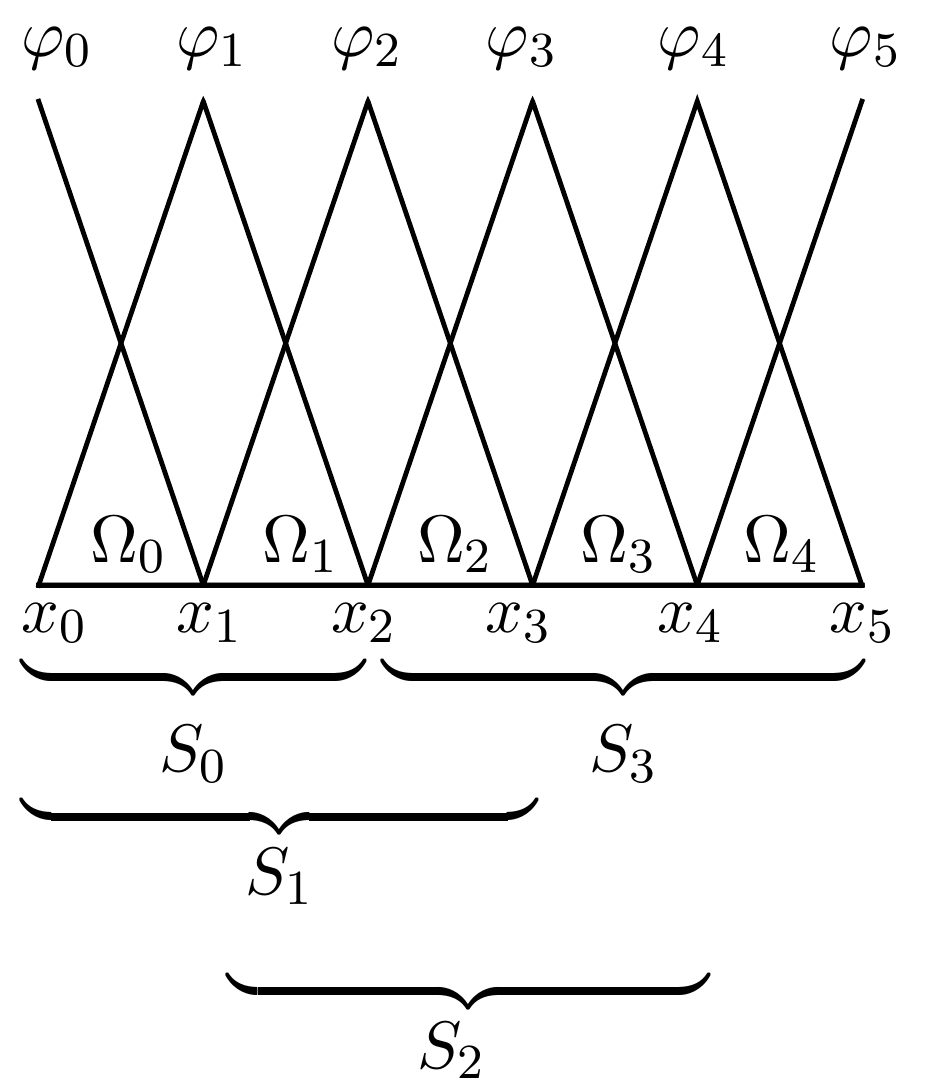
\includegraphics[width=5cm]{ex.pdf}}
% \put(0,0){$x_0$}
% \put(0,3.3){$\varphi_0$}
% \put(0.4,0.4){$\Omega_0$}
% \put(0.9,0){$x_1$}
% \put(0.9,3.3){$\varphi_1$}
% \put(1.4,0.4){$\Omega_1$}
% \put(1.8,0){$x_2$}
% \put(1.8,3.3){$\varphi_2$}
% \put(2.3,0.4){$\Omega_2$}
% \put(2.7,0){$x_3$}
% \put(2.7,3.3){$\varphi_3$}
% \put(3.25,0.4){$\Omega_3$}
% \put(3.7,0){$x_4$}
% \put(3.7,3.3){$\varphi_4$}
% \put(4.2,0.4){$\Omega_4$}
% \put(4.7,3.3){$\varphi_5$}
% \put(4.7,0){$x_5$}
% \put(0,-0.2){\makebox(2,0){$\underbrace{\hspace{2cm}}^{}$}}
% \put(0.8,-0.8){$S_0$}
% \put(0,-1){\makebox(3,0){$\underbrace{\hspace{3cm}}^{}$}}
% \put(1.3,-1.5){$S_1$}
% \put(1.1,-2){\makebox(3,0){$\underbrace{\hspace{2.8cm}}^{}$}}
% \put(2.3,-2.5){$S_2$}
% \put(2.5,-0.2){\makebox(2,0){$\underbrace{\hspace{2.8cm}}^{}$}}
% \put(3.3,-0.8){$S_3$}
% \end{picture}
% \end{center}
% \end{figure}
%
% lolo

\end{document}

